%
% File: chap01.tex
% Author: Victor F. Brena-Medina
% Description: Introduction chapter where the biology goes.
%
\let\textcircled=\pgftextcircled
\chapter{Methodology}
\label{chap:methodology}
In this chapter, the methodology has been clarified. For discussion convenience, there are a total of 3 sub-chapters under chapter 3, which we introduced. In section 3.1, we discussed the collected dataset; in section 3.2, we discussed data pre-processing; in section 3.3, we discussed proposed deep learning architectures.

\vspace{150mm}
%\vspace{2mm}

%=======
\section{Introduction}
\label{sec:sec3_1}
This chapter outlines the proposed model and methodology for analyzing the genetic profiling between BT and its comorbidities. The study integrates bioinformatics and system biological techniques to process gene expression data of BT and its complications such as PCOS, hypothyroidism, hypogonadism, diabetes, cardiomyopathy and arrhythmia.

The methodology involves data preprocessing, genetic profiling, pathway enrichment, functional ontology, protein-protein and protein-drug interaction networks, phylogenetic analysis and validation analysis. These approaches aim to identify key biomarkers, therapeutic targets and evolutionary insights between the genes of BT and its comorbidities. The details of these analytical approaches are presented in the following sections.

\section{Overview of Analytical Approaches}
\label{sec:sec3_2}

This chapter show a standard analytical procedure to gain the genetic link between beta-thalassemia and its comorbidities by analyzing the microarray and mRNA sequence datasets. We have used Gene Expression Omnibus (GEO) datasets for each diseases where each datasets has two groups: normal tissue (healthy or control samples) and malignant tissue (affected samples). Comparing these normal and malignant tissues by using Benjamini-Hochberg method to make sure that the significant genes are reliable and control the false discovery rate by adjusting p-value. A Limma package of R language to identify differentially expressed genes (DEGs) between BT and PCOS, T2D, hypothyroidism, hypogonadism, ACM, arrhythmia respectively. After applying the Benjamini-Hochberg correction to control the false discovery rate, this study applies statistical thresholds to differentiate up-regulated and down-regulated genes. And then by finding common DEGs, disease-gene network was constructed to visualize their co-relations. This study performed ontological analysis, pathway analysis, PPI, PDI, phylogenetic analysis and their respective networks. After that it performed validation analysis using gold benchmark datasets including dbGaP and OMIM. 

A working flowchart representing this quantitative method in Figure 3-1.

\begin{figure}[H]
\begin{center}
    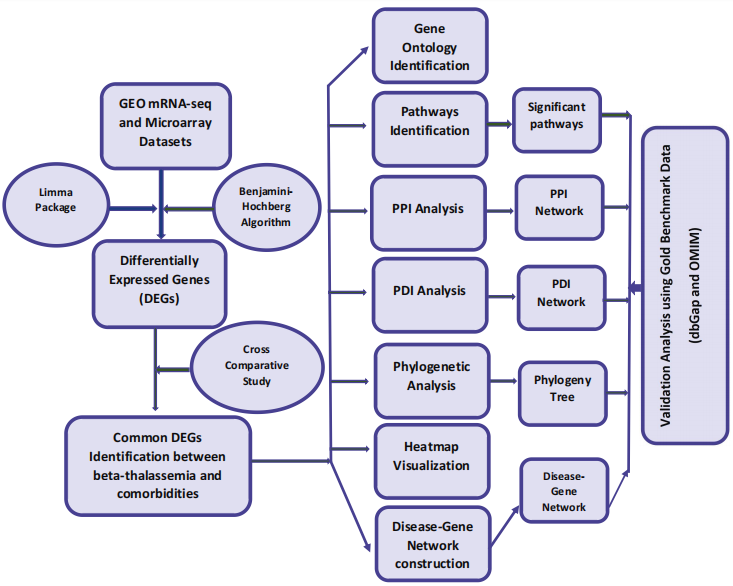
\includegraphics[width=15cm]{./fig/p1.PNG}
\end{center}
\caption{Working flow diagram of this investigation}
\label{fig:dataset_mass_images}
\end{figure}

\section{Dataset Information}
\label{sec:sec3_2}

This study investigated mRNA-seq datasets for BT, PCOS, hypothyroidism, ACM, and arrhythmia, and microarray datasets for T2D and hypogonadism, available in Gene Expression Omnibus (GEO), which is maintained by National Center for Biotechnology Information (NCBI) \cite{b3}, to identify the genetic link between beta-thalassemia and its comorbidities. Each and every datasets has two group normal tissue and malignant or affected tissue. This work compares these normal and malignant samples to indicate which genes are expressed differentially. Those differences can then point out the possible genetic links between BT and its comorbidities.

For BT, GSE117221 GEO mRNA-seq dataset are selected which has total 49 samples. 17 samples are normal tissue that means healthy patient and 32 samples are malignant tissue where (15 samples for thalassemia intermediate and 17 samples for thalassemia major) both type of patients are either female or male. 

For T2D, GSE25724 expression profiling by array genes are selected with 13 samples where 7 samples for type 2 diabetes patients and 6 samples for non-diabetic patients. 
GSE216609 mRNA-seq datasets are selected for PCOS with total 7 samples where 4 sample for control and 3 samples for polycystic ovary syndrome.

With 8 samples GSE176153 GEO mRNA genes are selected for hypothyroidism where 4 samples for healthy patients and 4 samples for malignant patients for both male and female. 
For ACM RNA-seq datasets are selected from NCBI. Its GEO accession is GSE233780 with 12 samples where 6 samples for ACM and other 6 for healthy control. 

GSE26966 GEO microarray datasets are used for hypogonadism with 23 samples where 9 samples for normal pituitary and 14 samples for gonadotrope tumor. 

For arrhythmia GSE175944 mRNA-seq datasets are collected which introduced the most common arrhythmia is atrial fibrillation with 6 samples where 3 samples for control patient and 3 samples for case samples. 

Table 3-1 provides a detailed representation of datasets including GEO accession id, Gender (no. of male and no. of female), samples (divided into case and control groups), associated diseases and source name that indicates the tissue type, cell type or experimental conditions.

% \begin{table}[h]
% \caption{Augmentation Parameters}
% \begin{center}
% \begin{tabular}{|c|c|c|}
% \hline
% \textbf{Augmentation Technique} & \textbf{Parameter} & \textbf{Value} \\
% \hline
% \multirow{4}{*}{RGB Shift} 
% & R Shift & 5 \\ \cline{2-3}
% & G Shift & 5 \\ \cline{2-3}
% & B Shift & 5 \\ \cline{2-3}
% & Probability & 0.7 \\
% \hline
% Random Brightness & Probability & 0.7 \\
% \hline
% \multirow{2}{*}{Motion Blur} 
% & Blur & 7 \\ \cline{2-3} & Probability & 0.7 \\
% \hline
% \end{tabular}
% \caption{Augmentation Parameters}
% \label{tab:augmentation}
% \end{center}
% \end{table}

\vspace*{-\parskip} % Remove extra paragraph spacing before table
\begin{longtable}{|p{0.5cm}|p{2.0cm}|p{1.4cm}|p{1.8cm}|p{2.0cm}|p{2.3cm}|p{2.0cm}|}
\caption{Representation of Datasets Information} \label{tab:3.1} \\
\hline
\textbf{S. No.} & \textbf{Disease Name} & \textbf{GEO Accession Id.} & \textbf{Gender (Male + Female)} & \textbf{Sample (Case + Control)} & \textbf{Disease status (case, control)} & \textbf{Source Name} \\
\hline
\endfirsthead
\caption[]{Representation of Datasets Information (Continued)} \\
\hline
\textbf{S. No.} & \textbf{Disease Name} & \textbf{GEO Accession Id.} & \textbf{Gender (Male + Female)} & \textbf{Sample (Case + Control)} & \textbf{Disease status (case, control)} & \textbf{Source Name} \\
\hline
\endhead
\hline
\endfoot
1 & Beta-thalassemia & GSE-117221 & 49 total, (23 + 26) & 49 samples, (32 + 17) & Thalassemia intermediate (TI) and Thalassemia major (TM), and Healthy patient & Healthy-ErPCs, TI-ErPCs, TM-ErPCs \\
\hline
2 & T2D & GSE-25724 & 13 total, (07 + 06) & 13 samples, (06 + 07) & Non-diabetic, and Type 2 diabetes & Human islets, non-diabetic and Human islets, diabetic \\
\hline
3 & PCOS & GSE-216609 & 07 total, (07 female) & 07 samples, (03 + 04) & Control, and PCOS & Cumulus granule cells \\
\hline
4 & Hypothyroi-dism & GSE-176153 & 08 total, (02 + 06) & 08 samples, (04 + 04) & Control, and Hypothyroidism & Whole blood \\
\hline
5 & ACM & GSE-233780 & 12 total, (10 + 02) & 12 samples, (06 + 06) & ACM, and Healthy control & Cardiac mesenchymal stromal cells \\
\hline
6 & Hypogona-dism & GSE-26966 & 23 total, (12 + 11) & 23 samples, (09 + 14) & Normal pituitary (NP), and Gonadotrope tumor (GT) & NP at autopsy within 2--18 hr. of death, and GT at time of transsphenoidal surgery \\
\hline
7 & Arrhythmia & GSE-175944 & Not mentioned & 06 samples, (03 + 03) & Control, and PITX2 knockout & Cell line of human induced pluripotent stem cells (hiPSC) \\
\hline
\end{longtable}


\newpage
\section{Methodology}
\label{sec:sec3_4}

This section provides a detailed overview of the methodology applied in this study. Different analytical approaches have been applied to investigate the genetic profiling of beta-thalassemia and its associated comorbidities. The process includes data collection, preprocessing, identification of important functional genes, enrichment analysis, and network-based evaluations such as protein-protein and protein-drug interactions. Additionally, evolutionary relationships has been incorporated to strengthen the findings. By combining these diverse methods, the study aims to ensure a comprehensive and reliable analysis framework that captures both the molecular and clinical perspectives of beta-thalassemia.

\subsection{Selection of mRNA-seq and Microarray Datasets}
\label{sec:sec3_4_1}
For BdSL classification, this study used pre-trained convolutional neural networks, ResNet-50 for feature extraction and evaluating two classifiers SVM (Support Vector Machine) and CNN (Convolutional Neural Network) for the final classification job.

For this study, a reliable and relevant data was selected for investigating the genetic association between BT and its comorbidities. Two types of datasets were utilized that are mRNA-seq datasets and microarray datasets which were selected from the Gene Expression Omnibus (GEO), a public functional genomics data repository maintained by the National Center for Biotechnology Information (NCBI) [new ref].

\begin{itemize}
    \item mRNA-seq datasets (gene expression that is profiling by high throughput sequencing ) were selected for BT, PCOS, hypothyroidism, ACM and arrhythmia. These datasets provide a comprehensive view of transcriptional expression.
    \item Microarray datasets (gene expression that is profiling by array) were selected for T2D and hypogonadism from GEO. Microarray datasets remain valuable for differential expression analysis for experimental designs.
\end{itemize}

% \begin{figure}[H]
% \begin{center}
%     % First row of images
%     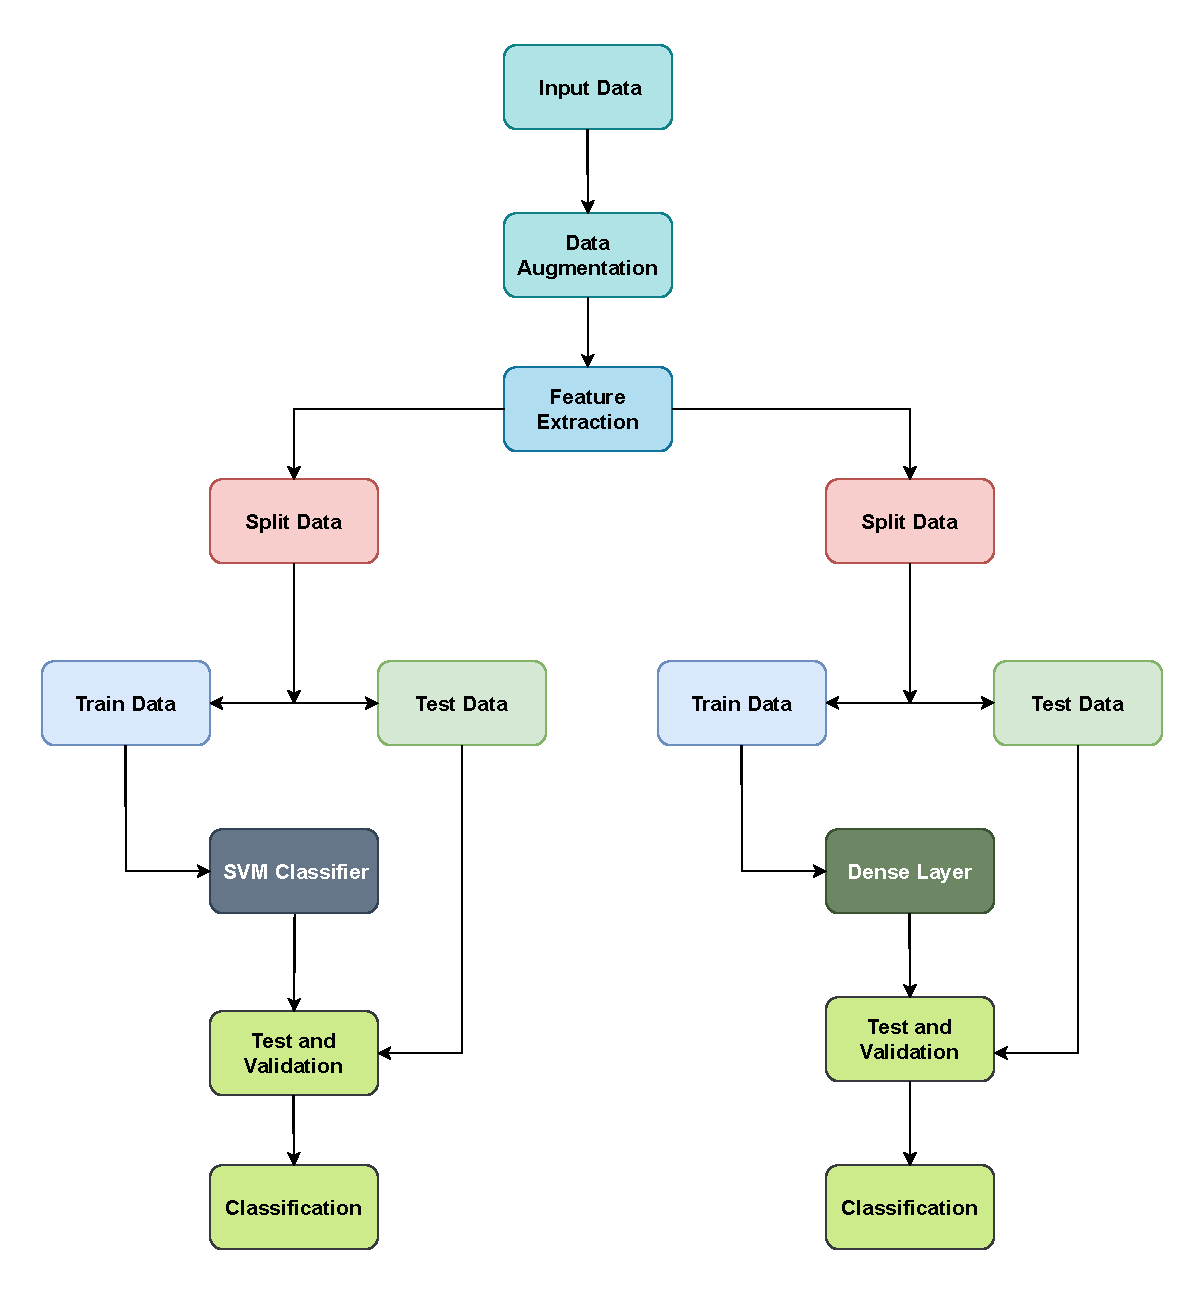
\includegraphics[width=15cm]{./fig/methodology.pdf}
% \caption{Procedure of methodological steps.}
% \label{tab:augmentation}
% \end{center}
% \end{figure}


\newpage
\subsection{Differential Gene Expression Analysis}
\label{sec:sec3_4_2}
Differential gene expression analysis is a base of bioinformatics for understanding the molecular and genetic inter-relations of complex diseases like beta-thalassemia and its comorbidities. In this study, we performed gene expression analysis on microarray and mRNA-seq datasets to identify differentially expressed genes (DEGs) between case disease and control samples for BT, PCOS, hypothyroidism, hypogonadism, T2D, ACM and arrhythmia. The analysis was conducted using the GEO2R tool on NCBI Gene Expression Omnibus (GEO) website and the Limma package in R which are widely used for strong statistical frameworks.

\begin{figure}[H]
\begin{center}
\begin{tikzpicture}[
  process/.style={rectangle, minimum width=3cm, minimum height=1cm, text centered, draw=black, fill=blue!20},
  decision/.style={diamond, minimum width=2.5cm, minimum height=1cm, text centered, draw=black, fill=green!20},
  startstop/.style={ellipse, minimum width=3cm, minimum height=1cm, text centered, draw=black, fill=red!20},
  arrow/.style={-Stealth, thick},
  label/.style={font=\small, midway, auto}
]

% Nodes
\node[startstop] (start) {Start: DEG Analysis};
\node[process, below of=start, yshift=-1cm] (data) {Datasets: Microarray, mRNA-seq (GEO)};
\node[decision, below of=data, yshift=-3.0cm] (samples) {Case vs. Control Samples};
\node[process, below of=samples, yshift=-3.0cm] (tools) {Tools: GEO2R, Limma (R)};
\node[process, below of=tools, yshift=-1cm] (analysis) {DEG Analysis};
\node[process, below of=analysis, yshift=-1cm] (results) {DEGs for BT, PCOS, etc.};
\node[startstop, below of=results, yshift=-1cm] (end) {End: Molecular Insights};
\node[process, right of=samples, xshift=8cm, align=left, minimum width=2cm] (diseases) {BT, PCOS, Hypothyroidism,\\ Hypogonadism, T2D, ACM, Arrhythmia};

% Arrows with labels
\draw[arrow] (start) -- (data) node[label, right] {Begin};
\draw[arrow] (data) -- (samples) node[label, right] {Data Input};
\draw[arrow] (samples) -- (tools) node[label, right] {Sample Classification};
\draw[arrow] (tools) -- (analysis) node[label, right] {Statistical Analysis};
\draw[arrow] (analysis) -- (results) node[label, right] {Identify DEGs};
\draw[arrow] (results) -- (end) node[label, right] {Output};
\draw[arrow, dashed] (samples) -- (diseases) node[label, above] {Diseases Studied};

\end{tikzpicture}
\caption{Workflow for Differential Gene Expression Analysis of Beta-Thalassemia and Comorbidities.}
\label{fig:deg-workflow}
\end{center}
\end{figure}

\vspace*{-\parskip} % Counteract extra paragraph spacing
\textbf{Data Pre-processing and Normalization}
\vspace{7mm}

To reduce experimental differences and keep the data consistent, gene expression values in each dataset were normalized using the Z-score method. This approach standardizes the expression values to make them comparable across different samples~\cite{zscore_ref}. The Z-score transformation for a gene expression value is calculated as:
\begin{equation}
z_{ij} = \frac{x_{ij} - \mu_i}{\sigma_i}
\label{eq:zscore}
\end{equation}
where:
\begin{itemize}
    \item $z_{ij}$: Normalized gene expression value for gene $i$ in sample $j$,
    \item $x_{ij}$: The value of gene expression $i$ in sample $j$,
    \item $\mu_i$: Mean value of gene expression $i$ in all samples,
    \item $\sigma_i$: The standard deviation of gene expression values $i$.
\end{itemize}

The normalization method was applied to both microarray (for T2D and hypogonadism) and mRNA-seq (for BT, hypothyroidism, PCOS, ACM, and arrhythmia) datasets to ensure reliable identification of differentially expressed genes (DEGs).

\vspace{8mm}
\textbf{Statistical Analysis for DEG Identification}
\vspace{5mm}

We identified the differentially expressed genes (DEGs) by applying the Benjamini-Hochberg (BH) correction method, which minimizes false positives by controlling the false discovery rate (FDR). The BH formula is:
\begin{equation}
\text{BH adjusted } p\text{-value} = \frac{i}{m} Q
\label{eq:bh_formula}
\end{equation}
where:
\begin{itemize}
    \item $i$: Rank of individual $p$-value,
    \item $m$: Total number of tests,
    \item $Q$: False discovery rate threshold.
\end{itemize}

The adjusted $p$-value threshold of BH was set to $\leq 0.05$ to ensure statistical significance. These genes were classified based on the $\log_2$ fold change ($\log FC$) values by applying the following conditions:
\begin{itemize}
    \item To identify up-regulated genes: $\textbf{log FC} > \text{threshold}$,
    \item To identify down-regulated genes: $\textbf{log FC} < \text{threshold}$.
\end{itemize}

These threshold values were used to identify significant DEGs between case and control groups.

\vspace*{-\parskip} % Counteract extra paragraph spacing
\subsection{Gene Diseases Network Analysis}
\label{sec:sec3_4_3}

This study constructed Disease-Gene Networks (DGNs) using a neighborhood-based benchmarking and topological approach to investigate the genetic associations between beta-thalassemia and its comorbidities. These networks of up- and down-regulated genes show the relationships between diseases and differentially expressed genes (DEGs), providing a visual framework to identify shared genetic signatures.

Each node represents either a disease or a gene, where diseases are source nodes and their associated genes are target nodes in the DGN network. This disease-gene connection forms a bipartite graph. A connection exists if at least one significant DEG is shared between a disease and beta-thalassemia. Let \(D\) represent the set of diseases and \(Z\) represent the set of dysregulated genes identified from the gene expression analysis, where a gene \(z \in Z\) is connected to a disease \(d \in D\) if \(z\) is significantly dysregulated in the dataset for \(d\). If associated diseases \(d_1\) and \(d_2\) have sets of significant dysregulated genes \(Z_1\) and \(Z_2\), respectively, then the number of shared genes is defined as:
\begin{equation}
|Z_1 \cap Z_2|
\label{eq:shared_genes}
\end{equation}

By using the Jaccard Coefficient, this study measured the similarity between disease pairs, which evaluates the overlap relative to the total unique genes. The edge weight or similarity score between diseases \(d_1\) and \(d_2\) is calculated as:
\begin{equation}
X(d_1, d_2) = \frac{|Z_1 \cap Z_2|}{|Z_1 \cup Z_2|}
\label{eq:jaccard}
\end{equation}
Here, \(|Z_1 \cap Z_2|\) represents the set of common DEGs, and \(|Z_1 \cup Z_2|\) represents the union of DEGs for the two diseases. The Jaccard Coefficient \(X(d_1, d_2)\) ranges from 0 to 1, where a higher value indicates greater similarity in the genetic profiles of the diseases~\cite{jaccard_ref}.

Two separate networks were constructed for up-regulated and down-regulated DEGs to show the distinct regulatory patterns. The DGNs were visualized and analyzed using the Cytoscape platform. Cytoscape enabled the mapping of disease-gene associations by optimizing the layouts to highlight connectivity patterns, such as hub genes across multiple comorbidities.

\vspace*{-\parskip} % Counteract extra paragraph spacing
\subsection{Pathway and Functional Association Analysis}
\label{sec:sec:sec3_4_4}

Pathway analysis involves the systematic identification of enriched biological pathways from sets of differentially expressed genes (DEGs) that are shared between beta-thalassemia and its comorbidities. This study identifies significant pathways using Enrichr, a public tool developed by the Ma'ayan Laboratory for Computational Systems Biology for gene set enrichment analysis (GSEA). Enrichr works by comparing input gene lists with collections of curated biological databases. The method applies statistical tests to measure significance, ensuring reliable and meaningful insights into the underlying molecular mechanisms.

A pathway is a sequence of molecular interactions that results in a specific change or product in a cell. It is a standard method for understanding the connections between complex diseases~\cite{pathway_ref}. We investigated dysregulated gene pathways across four databases using Enrichr: Reactome, KEGG, WikiPathways, and BioCarta.

\begin{enumerate}
    \item \textbf{Preparation of Input Gene Sets} \\
          Enrichr compares the input gene list against a reference set that includes all known annotated genes in the human genome (approximately 20,000--30,000), depending on each library. Using this background, it ensures that the analysis is fair and considers the full range of genes that could potentially be expressed.
    \item \textbf{Selection of Pathway Libraries} \\
          Enrichr compares the input gene list against multiple pathway-focused databases. This study selects four databases based on their relevance to biological processes:
          \begin{itemize}
              \item \textbf{KEGG} (Kyoto Encyclopedia of Genes and Genomes) provides correlated sets of genes involved in metabolic, signaling, and disease pathways.
              \item \textbf{Reactome} is an open-source database of manually curated biological pathways, focusing on reactions and interactions.
              \item \textbf{WikiPathways} is a community-curated resource with pathways linked to drug interactions and biological processes.
              \item \textbf{BioCarta} focuses on gene interaction models in signaling and metabolic pathways.
          \end{itemize}
\end{enumerate}

Using Enrichr, we analyzed the common DEGs identified from the cross-comparative analysis of beta-thalassemia and its comorbidities. Pathways were considered significant if their adjusted $p$-value was $\leq 0.05$, ensuring robust statistical reliability. The analysis identified key pathways for each comorbidity, such as GPCR ligand binding for PCOS, interferon gamma signaling for hypogonadism, and zinc homeostasis for arrhythmia, among others.

\vspace*{-\parskip} % Counteract extra paragraph spacing
\subsection{Gene Ontology Analysis}
\label{sec:sec3_4_5}

Gene Ontology (GO) analysis is a structured framework for describing genes by their molecular functions, biological processes, and cellular components, enabling a deeper understanding of their roles in disease mechanisms~\cite{go_ref}. In this study, we conducted GO analysis to explore the functional associations of common differentially expressed genes (DEGs) shared between beta-thalassemia and its comorbidities. The analysis was performed using Enrichr, a web-based enrichment tool developed by the Ma'ayan Laboratory, which queries gene sets against standardized ontology databases to identify significant functional terms~\cite{go_ref}.

\paragraph{GO Analysis Workflow}

The common DEGs identified through cross-comparative analysis of GEO datasets were used as input for Enrichr. We focused on two key ontology databases:
\begin{itemize}
    \item \textbf{GO Biological Process (GO Term)} categorizes genes based on their involvement in coordinated biological processes, such as signaling pathways or metabolic activities.
    \item \textbf{Human Phenotype Ontology (HP Term)} links genes to phenotypic abnormalities observed in diseases, facilitating the identification of clinical manifestations associated with DEGs.
\end{itemize}

\begin{figure}[h]
\centering
\begin{tikzpicture}[
    box/.style={rectangle, draw, rounded corners, minimum height=1cm, minimum width=7cm, text width=5cm, align=center, font=\small},
    arrow/.style={-Stealth, thick}
]
\node[box] (input) at (0,0) {Input DEGs from GEO datasets};
\node[box] (enrichr) at (0,-2) {Query Enrichr with GO Biological Process and HP Ontology};
\node[box] (output) at (0,-4) {Identify significant terms ($p \leq 0.05$)};
\draw[arrow] (input) -- (enrichr);
\draw[arrow] (enrichr) -- (output);
\end{tikzpicture}
\caption{Workflow for Gene Ontology (GO) analysis using Enrichr to identify significant functional terms associated with DEGs.}
\label{fig:go_workflow}
\end{figure}

\vspace*{-\parskip} % Counteract extra paragraph spacing
\subsection{Up and Down-regulated Identification}
\label{sec:sec3_4_6}

Downregulation is the process in which a cell reduces the expression level of a gene compared to a reference in response to an external variable. Upregulation refers to an increase in expression level compared to a reference. Here, the expression level indicates the abundance of biological components, such as RNA or protein~\cite{updown_reg_ref}. These changes are typically determined by comparing two groups: a reference or control sample, often healthy tissue, and a test sample, such as diseased or mutant tissue. The expression values of the test sample are compared against those of the reference sample to generate expression ratios, which is standard practice in gene expression analysis. These ratios are typically transformed into a logarithmic scale for easier interpretation. A positive log value indicates that the gene expression is higher in the test sample compared to the reference, indicating upregulation. A negative log value signifies reduced expression in the test sample relative to the reference, indicating downregulation. Thus, by comparing the expression profiles of two samples, it is possible to determine whether a gene is up- or down-regulated under specific conditions.

\begin{figure}[h]
\centering
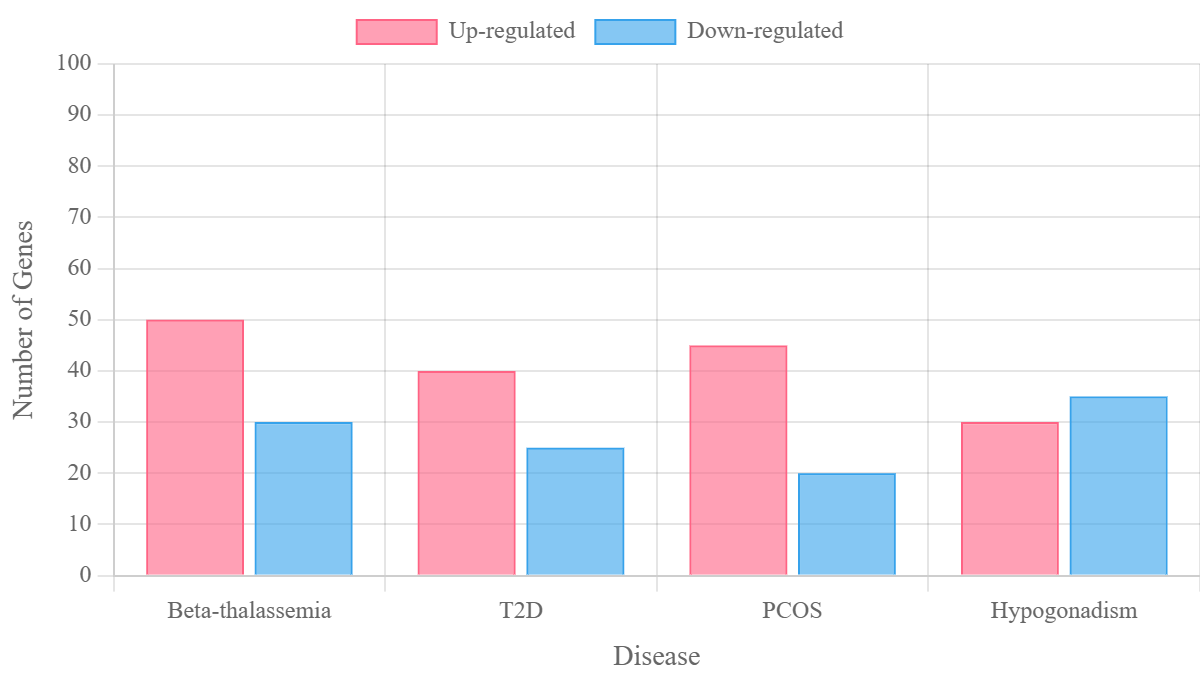
\includegraphics[width=0.95\textwidth]{./fig/disease}
\caption{Number of up- and down-regulated genes across diseases, identified by comparing expression levels between test and control samples using $\log_2$ fold change thresholds (e.g., $\log FC > 1$ for up-regulated, $\log FC < -1$ for down-regulated, $p \leq 0.05$).}
\label{fig:up_down_genes}
\end{figure}

\vspace*{-\parskip}
\subsection{Common Dysregulated Genes}
\label{sec:common_degs}

This study identified common differentially expressed genes (DEGs) shared between beta-thalassemia (BT) and its comorbidities by using statistical analysis to explore genetic relationships among these diseases. We retrieved GEO datasets from NCBI for the diseases under investigation. To reject the null hypothesis, a statistical \( p \)-value of \( \leq 0.05 \) was used. For up-regulated gene identification, a threshold of \( |\log FC| \geq 1 \) was applied, and for down-regulated gene identification, a threshold of \( |\log FC| \leq -1 \) was used~\cite{common_deg_ref}. By performing an intersection set operation using the R \texttt{limma} package, we identified common genes between BT and its comorbidities. Using these datasets and methods, we obtained results that demonstrate the connections between BT and the selected diseases. Other detailed information is discussed in the next chapter.

\vspace*{-\parskip}
\subsection{Network Construction of PPI}
\label{sec:ppi_network}

Protein-Protein Interaction (PPI) analysis is a primary goal of systems biology, predicting protein functions and drug targets through molecular interactions~\cite{ppi_ref1}. These interactions are significant for driving cellular processes and mapping connections between beta-thalassemia (BT) and its comorbidities~\cite{ppi_ref2}. We constructed PPI networks to explore how proteins encoded by shared differentially expressed genes (DEGs) interact.

We used the STRING database, inputting common DEGs and setting a high confidence score of 0.9 for reliable interactions. The NetworkAnalyst platform, utilizing the Markov Clustering algorithm, facilitated clustering of proteins based on connectivity. The resulting networks were visualized in Cytoscape, with proteins represented as nodes and interactions as edges.

Hub proteins were selected based on topological parameters, specifically a degree greater than 10. The distance between a pair of proteins (\( i, j \)) is defined as follows:
\begin{equation}
d(i,j) = 1 - \frac{|N_i \cap N_j|}{|N_i \cup N_j|}
\label{eq:protein_distance}
\end{equation}
where \( N_i \) and \( N_j \) are the neighbor sets of proteins \( i \) and \( j \), respectively.

\vspace*{-\parskip}
\subsection{Protein-Drug Interactions Network Analysis}
\label{sec:pdi_network}

The primary objective of this investigation is to identify potential therapeutic drug particles~\cite{pdi_ref1}. The Protein-Drug Interaction (PDI) network was constructed using NetworkAnalyst and prepared with the DrugBank database, which is designed for common genes of beta-thalassemia and its comorbidities. To explore potential therapeutic options for beta-thalassemia and its comorbidities, we constructed PDI networks. These networks map how proteins encoded by the shared differentially expressed genes (DEGs) interact with drug molecules, which is used to identify possible treatments~\cite{pdi_ref2}. Using systems biology-based strategies for studying protein-drug interactions~\cite{pdi_ref3}, the goal of this work was to identify potential drug targets capable of addressing the molecular mechanisms that connect these diseases.

\subsection*{Building the PDI Networks}

Firstly, we identified the common DEGs between beta-thalassemia and each comorbidity. These genes were input into the NetworkAnalyst platform, which integrates the DrugBank database to map interactions between proteins and known drug compounds~\cite{pdi_ref1}. DrugBank provides a comprehensive repository of drugs and their protein targets, including approved, experimental, and investigational compounds, which is used to ensure a broad scope of potential interactions.

\subsection*{Analytical Approach}

Following the systems biology framework outlined by Colinge et al. (2012)~\cite{pdi_colinge}, we analyzed the PDI network by:
\begin{itemize}
    \item Topological Analysis is used to identify hub proteins with multiple drug interactions by using metrics like degree (the number of connections) to prioritize potential therapeutic targets.
    \item Functional Mapping is used for cross-referenced protein functions to ensure drugs targeted biologically relevant proteins, such as those involved in immune response or signaling pathways linked to beta-thalassemia’s comorbidities.
    \item Drug Prioritization were ranked based on the number of protein targets and their relevance to disease pathways, ensuring focus on compounds with potential clinical applicability.
\end{itemize}
The PDI network helps us see which drugs might influence the proteins driving beta-thalassemia and its comorbidities.

\vspace*{-\parskip}
\subsection{Phylogenetic Analysis}
\label{sec:phylogenetic}

Phylogenetic analysis enhances the understanding of the evolutionary relationships among genes, proteins, and diseases~\cite{phy_ref1}. We constructed a phylogenetic tree for beta-thalassemia and its comorbidities to illustrate the associative relationships among them by using Molecular Evolutionary Genetics Analysis (MEGA) tools and FASTA sequences of nucleotide datasets from NCBI~\cite{phy_ref1}. The tree shows a strong evolutionary relationship between beta-thalassemia and hypogonadism as they belong to a common species.
We retrieved nucleotide sequences in FASTA format from the NCBI database for representative genes associated with beta-thalassemia and its comorbidities by selecting sequences based on their relevance to shared differentially expressed genes (DEGs). To ensure comprehensive coverage, we included multiple sequences per disease and prioritized those linked to key pathways like iron metabolism or endocrine signaling.
Following standard molecular phylogenetic protocols~\cite{phy_ref2}:
\begin{itemize}
    \item Sequence Alignment: Sequences were aligned using ClustalX to identify homologous regions, accounting for insertions, deletions, and substitutions. This step ensures accurate comparison for evolutionary inferences.
    \item Tree Construction: We used the Molecular Evolutionary Genetics Analysis (MEGA) software to generate phylogenetic trees. The Neighbor-Joining (NJ) method was employed, with the Kimura 2-parameter model for distance calculation to handle nucleotide substitutions~\cite{phy_ref3}.
\end{itemize}

\vspace*{-\parskip}
\subsection{Validation Analysis}
\label{sec:validation}

To ensure the reliability of our findings on the genetic links between beta-thalassemia and its comorbidities, we conducted a validation analysis using gold-standard biomedical databases. This step confirms that the DEGs and their disease associations are consistent~\cite{val_ref1}. We used two benchmark databases, including dbGaP and OMIM from Enrichr tools, on the up-regulated and down-regulated genes of beta-thalassemia to validate our findings~\cite{val_ref1}:
\begin{itemize}
    \item dbGaP (Database of Genotypes and Phenotypes): This NCBI-hosted database contains genotype-phenotype relationships from large-scale genomic studies. We queried dbGaP with our shared DEGs to identify diseases with overlapping genetic profiles.
    \item OMIM (Online Mendelian Inheritance in Man): This comprehensive catalog of human genes and genetic disorders was used to verify whether our DEGs are linked to beta-thalassemia or its comorbidities in Mendelian or complex disease contexts.
\end{itemize}

\vspace*{-\parskip}
\subsection{Working Algorithm}
\label{sec:working_algorithm}

A systematic methodology outlines the entire operational process as a set of structured steps. The following guidelines offer a detailed summary of all procedures carried out in our research~\cite{algo_ref1}.

\vspace*{-\parskip}
\subsection{Algorithm}
\label{sec:algorithm}

\textbf{Input:} Microarray and mRNA-Seq GEO datasets. \\
\textbf{Output:} Differentially Expressed Genes (DEGs), Common DEGs, Disease-Gene Networks (DGNs), Signaling Pathways, Ontological Pathways, Protein-Protein Interactions (PPIs), Protein-Drug Interactions (PDIs), Phylogenetic Tree, and Validation Network.

\begin{enumerate}
    \item \textbf{Dataset Selection:}
    \begin{itemize}
        \item Selecting relevant Gene Expression Omnibus (GEO) datasets from the NCBI using disease-specific criteria.
    \end{itemize}
    \item \textbf{Differential Gene Expression Analysis:}
    \begin{itemize}
        \item For every dataset \( i = 1, 2, 3, \ldots, N \)
        \begin{enumerate}
            \item Load the datasets.
            \item Normalize datasets using Z-score transformation to ensure comparability.
            \item Create a case vs. control design matrix.
            \item Apply the R \texttt{Limma} package and GEO2R to compute DEGs using the Benjamini-Hochberg method.
            \item Filter DEGs based on adjusted \( p \)-value \( \leq 0.05 \).
            \item Modify \( |\log FC| \geq 1 \) for Upregulation and \( |\log FC| \leq -1 \) for Downregulation.
            \item Identify significant DEGs.
        \end{enumerate}
    \end{itemize}
    \item \textbf{Cross-Comparative Analysis:}
    \begin{itemize}
        \item Compare DEG gene sets between beta-thalassemia and each comorbidity including T2D, PCOS, ACM, hypothyroidism, hypogonadism, and arrhythmia to identify common up- and down-regulated genes.
        \item Use the Jaccard Coefficient to quantify similarity between gene sets.
    \end{itemize}
    \item \textbf{Some Analysis for Common DEGs:}
    \begin{itemize}
        \item Disease-Gene Networks (DGNs) construction.
        \item Enrichment analysis for significant signaling pathways.
        \item Enrichment analysis for Ontological pathways.
        \item PPI network construction.
        \item PDI network construction.
        \item Evolutionary phylogenetic Analysis.
        \item Plot these pathways in tabular form.
    \end{itemize}
    \item \textbf{Validation Analysis:}
    \begin{itemize}
        \item Build a validation network in Cytoscape.
    \end{itemize}
    \item \textbf{Results:}
    \begin{itemize}
        \item List of common DEGs.
        \item DGNs for up- and down-regulated genes.
        \item Heatmap Visualization.
        \item Enriched signaling and ontological pathways.
        \item PPI networks and hub proteins.
        \item PDI networks with potential drug targets.
        \item Phylogenetic tree showing disease relationships.
        \item Validated disease-gene associations.
    \end{itemize}
\end{enumerate}

\vspace*{-\parskip}
\subsection{Experimental Setup}
\label{sec:experimental_setup}

To conduct the genetic and molecular analysis of beta-thalassemia and its comorbidities, we used the following computational setup and tools:
\begin{itemize}
    \item \textbf{Hardware:}
    \begin{itemize}
        \item Device: Desktop PC
        \item Processor: Intel Core i5-7200U CPU @ 2.50GHz (2.71 GHz)
        \item RAM: 4.00 GB (3.26 GB usable)
        \item System: 64-bit Windows 10 Pro, Version 21H2, OS Build 19044.2006
    \end{itemize}
    \item \textbf{Software and Tools:}
    \begin{itemize}
        \item R Studio: For differential gene expression analysis using the \texttt{Limma} package.
        \item Cytoscape: For constructing and visualizing disease-gene and validation networks.
        \item MEGA: For phylogenetic tree construction.
        \item STRING: For protein-protein interaction (PPI) network analysis.
        \item Enrichr: For pathway and gene ontology enrichment analysis.
        \item Network Analyst: For PPI and protein-drug interaction (PDI) network construction with DrugBank integration.
    \end{itemize}
\end{itemize}

\vspace*{-\parskip}
\subsection{Conclusion}
\label{sec:conclusion}

This chapter outlined the methodology for investigating the genetic and molecular links between beta-thalassemia and its comorbidities. Using GEO datasets, we identified DEGs, constructed DGNs, performed pathway and GO enrichment, built PPI and PDI networks, conducted phylogenetic analysis, and validated findings with dbGaP and OMIM. The systematic approach, supported by tools like R, Cytoscape, Enrichr, STRING, NetworkAnalyst, and MEGA, ensures robust and reproducible results, setting the stage for detailed findings in Chapter 4.
